\documentclass[11pt]{article}

\usepackage[a4paper]{geometry}
\usepackage[utf8]{inputenc} % allow utf-8 input
\usepackage{makecell}
\usepackage{listings}
\usepackage{stackengine}
\usepackage{enumitem}
\usepackage{bbm}
\usepackage{amsmath}
\usepackage{bbold}
\usepackage[colorlinks=true,citecolor=blue,urlcolor=blue]{hyperref}%
\usepackage{url}            % simple URL typesetting
\usepackage{booktabs}       % professional-quality tables
\usepackage{amsfonts}       % blackboard math symbols
\usepackage{nicefrac}       % compact symbols for 1/2, etc.
\usepackage{microtype}      % microtypography
\usepackage[round]{natbib}
\usepackage{titling} % Customising the title section
\usepackage{graphicx}
\usepackage{caption}
\usepackage{subcaption}
\usepackage{multirow}
%% The amsthm package provides extended theorem environments
\usepackage{amssymb}
\usepackage{amsthm}
\usepackage{amsmath}
\usepackage{fancyvrb}
\usepackage{dsfont}
\usepackage{algorithm}
\usepackage{algorithmicx}
\usepackage{algpseudocode}
%\usepackage{stackengine}
\usepackage[toc,page]{appendix}
\usepackage{stmaryrd}
\usepackage{hyperref}% http://ctan.org/pkg/hyperref
\usepackage{cleveref}% http://ctan.org/pkg/cleveref
\usepackage{lipsum}%
  {
      \theoremstyle{plain}
      \newtheorem{assumption}{M}
      \newtheorem{lemma}{Lemma}
      \newtheorem{remark}{Remark}
      \newtheorem{prop}{Proposition}
      \newtheorem{assumption_saem}{ISAEM}
      \newtheorem{assumption_rm}{SA}
      \newtheorem{assumption_iem}{IEM}
      \newtheorem{assumption_imcem}{IMCEM}
      \newtheorem{assumption_expo}{E}
  }
\crefname{lemma}{Lemma}{Lemmas}
\crefname{assumption}{M}{assumption}
\usepackage{amssymb,amsthm,mathrsfs,amsfonts,dsfont}
\usepackage{mathtools}
\usepackage{xargs}
\usepackage{shortcuts}

\lstset{% setup listings 
        language=R,% set programming language 
        basicstyle=\ttfamily\small,% basic font style 
        keywordstyle=\color{blue},% keyword style 
        commentstyle=\color{blue},% comment style 
        numbers=left,% display line numbers on the left side 
        numberstyle=\scriptsize,% use small line numbers 
        numbersep=10pt,% space between line numbers and code 
        tabsize=3,% sizes of tabs 
        showstringspaces=false,% do not replace spaces in strings by a certain character 
        captionpos=b,% positioning of the caption below 
        breaklines=true,% automatic line breaking 
        escapeinside={(*}{*)},% escaping to LaTeX 
        fancyvrb=true,% verbatim code is typset by listings 
        extendedchars=false,% prohibit extended chars (chars of codes 128--255) 
        literate={"}{{\texttt{"}}}1{<-}{{$\leftarrow$}}1{<<-}{{$\twoheadleftarrow$}}1 
        {~}{{$\sim$}}1{<=}{{$\le$}}1{>=}{{$\ge$}}1{!=}{{$\neq$}}1{^}{{$^{\wedge}$}}1,% item to replace, text, length of chars 
        alsoletter={.<-},% becomes a letter 
        alsoother={$},% becomes other 
        otherkeywords={!=, ~, $, \&, \%/\%, \%*\%, \%\%, <-, <<-, /},% other keywords 
        deletekeywords={c}% remove keywords 
} 





\title{Doc: extension of the saemix R package} 

\author{%
\textsc{Belhal Karimi}\\
\normalsize  CMAP, Ecole Polytechnique, Universite Paris-Saclay, 91128 Palaiseau, France\\ % Your institution
\normalsize \href{mailto:belhal.karimi@polytechnique.edu}{belhal.karimi@polytechnique.edu} % Your email address
}
\date{\today} % Leave empty to omit a date

\begin{document}


\maketitle



% !TEX root = main.tex


\section{Example}
\subsection{Noncontinuous data models}
SAEMIX can also be used for noncontinuous data models. Noncontinuous data models include categorical data models \citep{savic, agresti}, time-to-event data models \citep{mbogning, andersen}, or count data models \citep{savic}.

A categorical outcome $y_{ij}$ takes its value in a set $\{1, \dots, L\}$ of $L$ categories. Then, the model is defined by the conditional probabilities $\left(\mathbb{P}(y_{ij} = \ell | \psi_i),1 \leq \ell \leq L\right)$, that depend on the vector of individual parameters $\psi_i$ and may be a function of the time $t_{ij}$.

In a time-to-event data model, the observations are the times at which events occur. An event may be one-off (e.g., death, hardware failure) or repeated (e.g., epileptic seizures, mechanical incidents).
To begin with, we consider a model for a one-off event. The survival function $S(t)$ gives the probability that the event happens after time $t$:
\begin{equation}\label{survival}
S(t)  \triangleq \mathbb{P}(T >t) = \exp\left\{-\int_{0}^{t}h(u)\textrm{d}u\right\}\eqs,
\end{equation}
where $h$ is called the hazard function. 
In a population approach, we consider a parametric and individual hazard function $h(\cdot,\psi_i)$.

The random variable representing the time-to-event for individual $i$ is typically written $T_i$ and may possibly be right-censored. Then, the observation $y_i$ for individual $i$ is
\begin{equation}
    y_i = \left\{
    \begin{array}{ll}
        T_i & \mbox{if } T_i \leq \tau_c \\
        "T_i > \tau_c" & \mbox{otherwise}\eqs,
    \end{array}
\right.
\end{equation}
where $\tau_c$ is the censoring time and $"T_i > \tau_c"$ is the information that the event occurred after the censoring time. 


\subsection{A Repeated Time-Eo-Event Model}
\subsubsection{The model}

For repeated event models, times when events occur for individual $i$ are random times $(T_{ij}, 1\leq j \leq n_i)$  for which conditional survival functions can be defined:
\begin{equation}
\mathbb{P}(T_{ij} > t|T_{i(j-1)}=t_{i(j-1)}) = \exp\left\{-\int_{t_{i(j-1)}}^{t}h(u, \psi_i)\textrm{d}u\right\}\eqs.
\end{equation}
Here, $t_{ij}$ is the observed value of the random time $T_{ij}$.
If the last event is right censored, then the last observation $y_{i,n_i}$ for individual $i$ is the information that the censoring time has been reached $"T_{i,n_i} > \tau_c"$. The conditional pdf of $y_i = (y_{ij},1\leq n_i)$ reads (see \citep{laviellebook} for more details)
\begin{equation} \label{pdf_tte}
\dens(y_i |\psi_i) = \exp\left\{-\int_{0}^{\tau_c}h(u, \psi_i)\textrm{d}u \right\} \prod_{j=1}^{n_i-1} h(t_{ij},\psi_i)\eqs.
\end{equation}
\subsubsection{Numerical Application}
In this section, we consider a Weibull model for time-to-event data \citep{laviellebook, zhang}. For individual $i$, the hazard function of this model is:
\begin{align}\label{weibullmodel}
& h(t, \psi_i) = \frac{\beta_i}{\lambda_i}\left(\frac{t}{\lambda_i}\right)^{\beta_i-1}\eqs.
\end{align}
Here, the vector of individual parameters is $\psi_i = (\lambda_i, \beta_i)$. These two parameters are assumed to be independent and  lognormally distributed:
\begin{align} \label{indivtte}
& \log(\lambda_i) \sim \mathcal{N}(\log(\lambda_{\rm pop}), \omega^2_{\lambda})\eqs,\\
& \log(\beta_i) \sim \mathcal{N}(\log(\beta_{\rm pop}), \omega^2_{\beta})\eqs.
\end{align}
Then, the vector of population parameters is $\theta = (\lambda_{\rm pop}, \beta_{\rm pop}, \omega_{\lambda}, \omega_{\beta})$.

Repeated events were generated using simulx (mlxR package in R), for $N=100$ individuals, using the Weibull model \eqref{weibullmodel} with $\lambda_{\rm pop} = 10$, $\omega_{\lambda} = 0.3$, $\beta_{\rm pop} = 3$ and $\omega_{\beta} = 0.3$ and assuming a right censoring time $\tau_c = 20$.

The following code was used in R to run this example:

\begin{lstlisting}
library(saemix)
data(tte.saemix)
saemix.data<-saemixData(name.data=tte.saemix,header=TRUE,sep=" ",na=NA, name.group=c("id"),name.response=c("y"),name.predictors=c("time","y"), name.X=c("time"))

timetoevent.model<-function(psi,id,xidep) {
T<-xidep[,1]
N <- nrow(psi)
Nj <- length(T)
censoringtime = 20
lambda <- psi[id,1]
beta <- psi[id,2]
init <- which(T==0)
cens <- which(T==censoringtime)
ind <- setdiff(1:Nj, append(init,cens))
hazard <- (beta/lambda)*(T/lambda)^(beta-1)
H <- (T/lambda)^beta
logpdf <- rep(0,Nj)
logpdf[cens] <- -H[cens] + H[cens-1]
logpdf[ind] <- -H[ind] + H[ind-1] + log(hazard[ind])
return(logpdf)
}

saemix.model<-saemixModel(model=timetoevent.model,description="time model",type="likelihood",
psi0=matrix(c(2,1),ncol=2,byrow=TRUE,dimnames=list(NULL,
c("lambda","beta"))),
transform.par=c(1,1),covariance.model=matrix(c(1,0,0,1),ncol=2,
byrow=TRUE))


saemix.options<-list(map=F,fim=F,ll.is=F, nb.chains = 1, nbiter.saemix = c(200,100),displayProgress=TRUE,save.graphs=FALSE)


saemix.fit<-saemix(model,saemix.data,saemix.options)


\end{lstlisting}

Figure \ref{pop_tte} shows the convergence of the population parameters for this example. The results are summed up in the following table:

\begin{lstlisting}
----------------------------------------------------
----                  Results                   ----
----------------------------------------------------
-----------------  Fixed effects  ------------------
----------------------------------------------------
     Parameter Estimate
[1,] lambda    5.0     
[2,] beta      2.8     
----------------------------------------------------
-----------  Variance of random effects  -----------
----------------------------------------------------
       Parameter     Estimate
lambda omega2.lambda 0.039   
beta   omega2.beta   0.921   
----------------------------------------------------
------  Correlation matrix of random effects  ------
----------------------------------------------------
              omega2.lambda omega2.beta
omega2.lambda 1             0          
omega2.beta   0             1 
\end{lstlisting}



\begin{figure}[thp]
\begin{center}
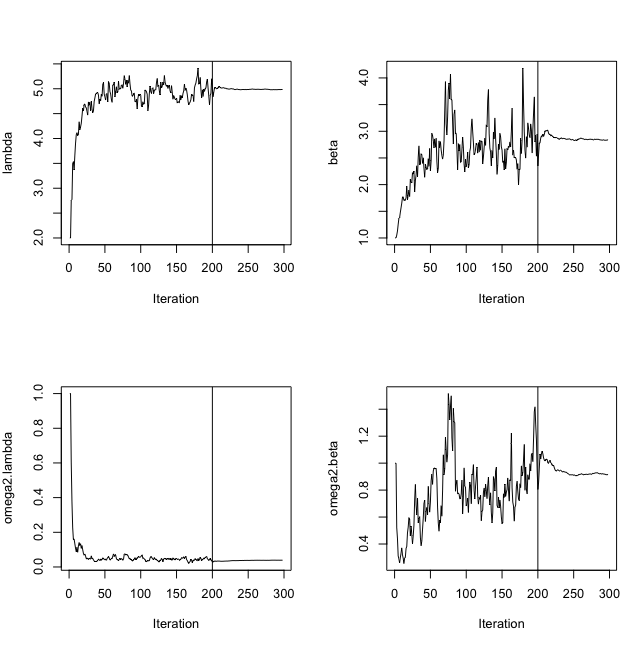
\includegraphics[width=\textwidth]{images/popparam_tte.png}
\caption{Time-to-event data modelling: convergence of the empirical quantiles of order 0.1, 0.5 and 0.9 of $\dens(\psi_i | y_i ; \theta)$ for a single individual. The reference MH algorithm is in blue and the nlme-IMH is in red.}
\label{pop_tte}
\end{center}
\end{figure}

\subsection{A Categorical data model with regression variables}
\subsubsection{The model}

Assume now that the observed data takes its values in a fixed and finite set of nominal categories $\{c_1, c_2,\ldots , c_K\}$. Considering the observations $(y_{ij},\, 1 \leq j \leq n_i)$ for any individual i as a sequence of conditionally independent random variables, the model is completely defined by the probability mass functions $\mathbb{P}(y_{ij}=c_k | \psi_i)$ for $k=1,\ldots, K$ and $1 \leq j \leq n_i$. For a given $(i,j)$, the sum of the K probabilities is $1$, so in fact only $K-1$ of them need to be defined. In the most general way possible, any model can be considered so long as it defines a probability distribution, i.e., for each k, $\mathbb{P}(y_{ij}=c_k | \psi_i) \in [0,1]$, and $\sum_{k=1}^{K} \mathbb{P}(y_{ij}=c_k | \psi_i) =1$. Ordinal data further assume that the categories are ordered, i.e., there exists an order $\prec$ such that

$$c_1 \prec c_2,\prec \ldots \prec c_K $$.

We can think, for instance, of levels of pain $(low \prec moderate \prec severe)$ or scores on a discrete scale, e.g., from 1 to 10. Instead of defining the probabilities of each category, it may be convenient to define the cumulative probabilities $\mathbb{P}(y_{ij} \preceq c_k | \psi_i)$ for $k=1,\ldots ,K-1$, or in the other direction: $\mathbb{P}(y_{ij} \succeq c_k | \psi_i)$ for $k=2,\ldots, K$. Any model is possible as long as it defines a probability distribution, i.e., it satisfies

$$0\leq\prob(y_{ij}\prec c_1|\psi_i)\leq\prob(y_{ij}\prec c_2|\psi_i)\leq \cdots \leq\prob(y_{ij}\prec c_K|\psi_i)=1$$
It is possible to introduce dependence between observations from the same individual by assuming that $(y_{ij},\,j=1,2,\ldots,n_i)$ forms a Markov chain. For instance, a Markov chain with memory 1 assumes that all that is required from the past to determine the distribution of $y_{ij}$ is the value of the previous observation $y_{i,j-1}$., i.e., for all $k=1,2,\ldots ,K$,

$$\prob(y_{ij}=c_k|y_{i,j-1},y_{i,j-2},y_{i,j-3},…,\psi_i)=\prob(y_{ij}=c_k|y_{i,j-1},\psi_i)$$

\subsubsection{Numerical application}

In this example, observations are ordinal data that take their values in ${0, 1}$
Odds ratio are used in this example to define the model
$$\logit(\prob(y_{ij} = k))= \log(\prob(y_{ij}= k) / [1–\prob(y_{ij}= k)])$$
where

\begin{align}
& \logit(\prob(y_{ij} =  0))= \theta_{i,1} + \theta_{i,2} \Time + \theta_{i,3} \dose
\end{align}
where Dose and Time are the two regression variables. 

Here, the vector of individual parameters is $\psi_i = (\theta_{i,1},\theta_{i,2},\theta_{i,3})$. These three parameters are assumed to be independent and  normally distributed:
\begin{align} \label{indivtte}
& \theta_{i,1} \sim \mathcal{N}(\theta_{\rm pop,1}, \omega^2_{1})\eqs,\\
& \theta_{i,1} \sim \mathcal{N}(\theta_{\rm pop,2}, \omega^2_{2})\eqs,\\
& \theta_{i,1} \sim \mathcal{N}(\theta_{\rm pop,3}, \omega^2_{3})
\end{align}
Then, the vector of population parameters is $\theta = (\theta_{\rm pop,1},\theta_{\rm pop,2},\theta_{\rm pop,1}, \omega_{1}, \omega_{2} ,\omega_{3})$.

\textbf{Data simulation:} Data is generated using $N=300$ and for all $i \in \inter$, $n_i=15$. For all $i \in \inter$ and $j \in \interi$, we take $d_{ij,1}= 1$,  $d_{ij,2} = -20 + (j-1)*5$ and for
$i \in \inter$ $d_{ij,3} = 10 \lceil 3i/N \rceil$.
The data is generated using the following values for the fixed and random effects $( \theta_{\rm pop,1} =-4, \theta_{\rm pop,2}= -0.5, \theta_{\rm pop,}=1,  \omega_1=0.3, \omega_2=0.2, \omega_3=0.2)$.

The figure \ref{fig:prob} shows the probability for each of the three subgroups:
\begin{figure}[thp]
\begin{center}
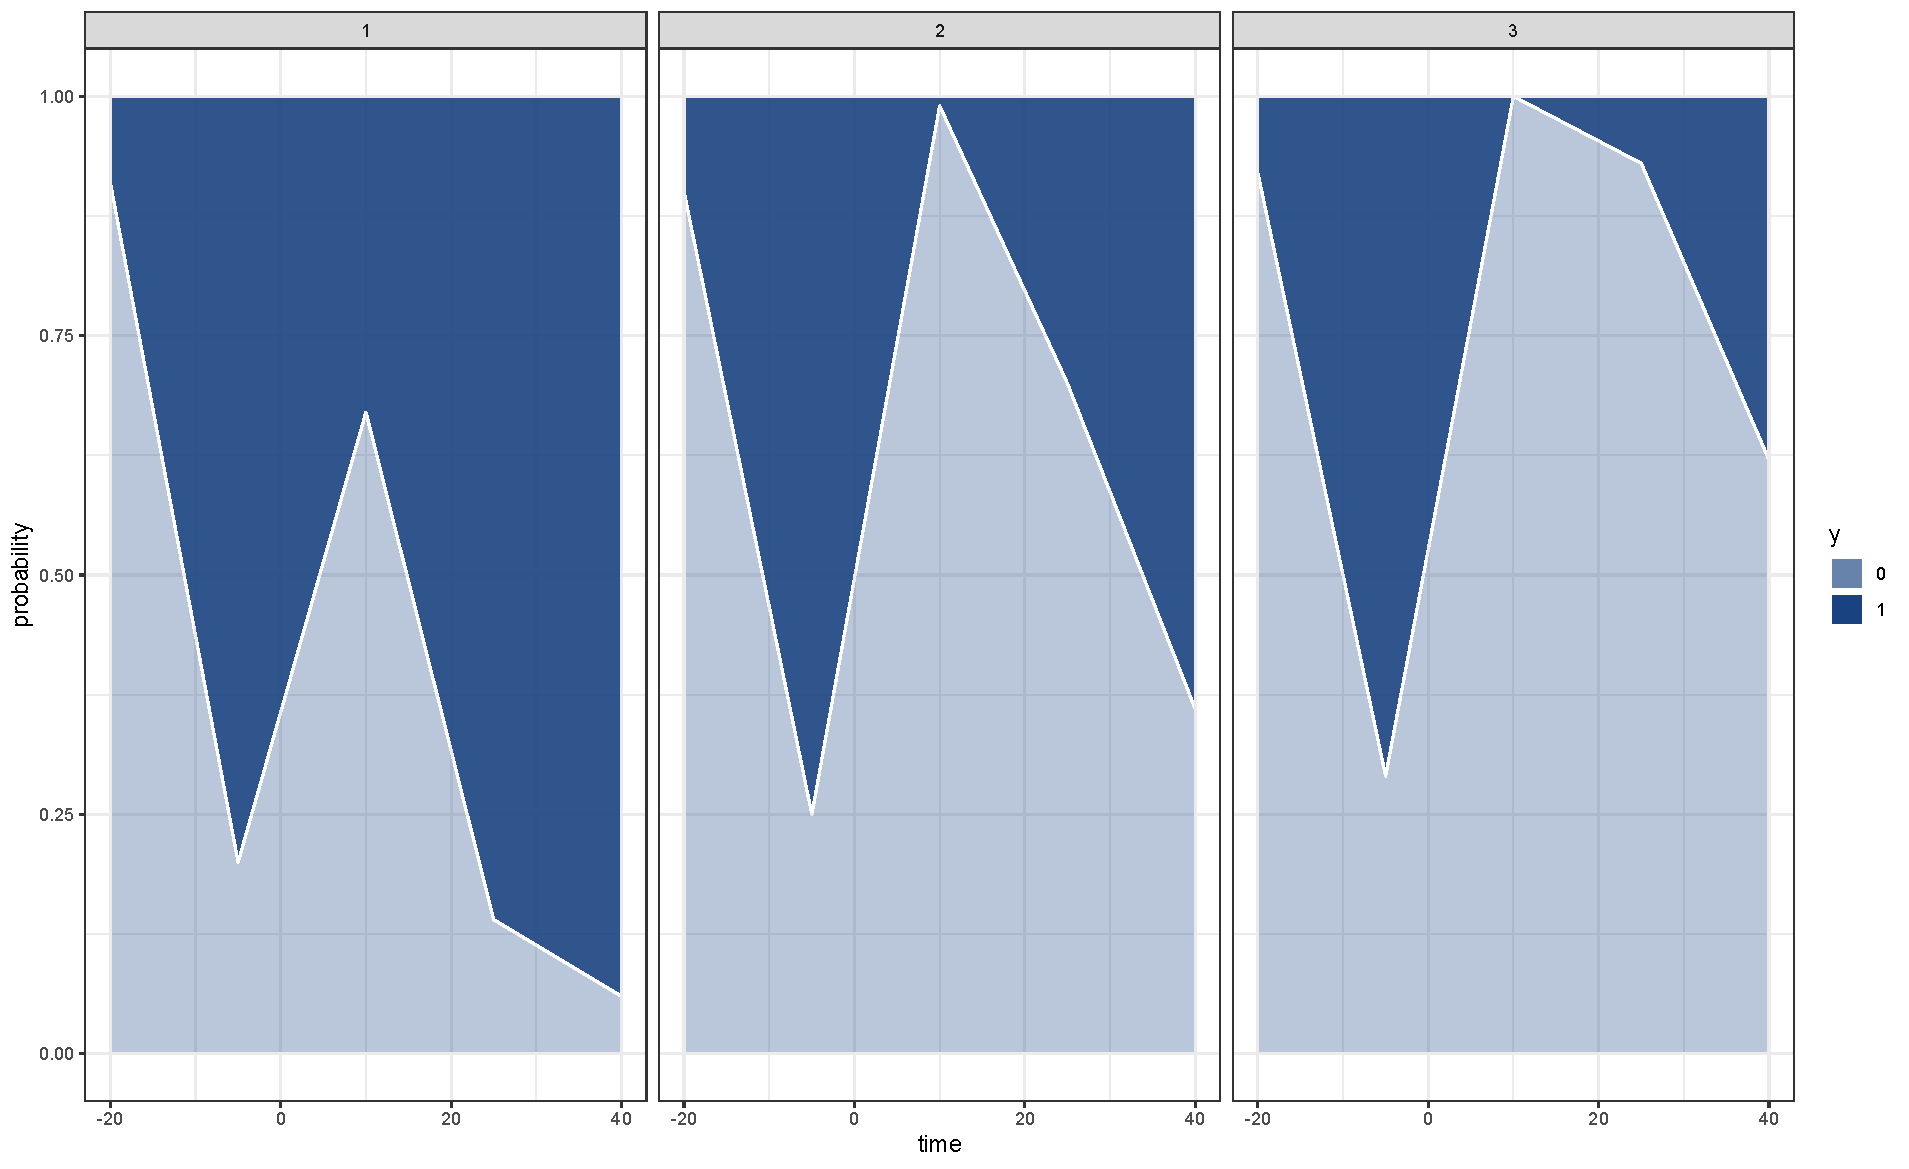
\includegraphics[width=\textwidth]{images/prob_class.pdf}
\caption{Prob.}
\label{fig:prob}
\end{center}
\end{figure}


The model is implemented in R as follows:

\begin{lstlisting}

cat.model<-function(psi,id,xidep) {
level<-xidep[,1]
dose<-xidep[,2]
time<-xidep[,3]

th1 <- psi[id,1]
th2 <- psi[id,2]
delta0 <- psi[id,3]

lm0 <- th1+th2*time + delta0*dose

D <- exp(lm0)+1
P0 <- exp(lm0)/D
P1 <- 1/D

P.obs = (level==0)*P0+(level==1)*P1

return(P.obs)
}


\end{lstlisting}
Then, the following code was used in R to run SAEM on this example:

\begin{lstlisting}
saemix.model<-saemixModel(model=cat_data.model,description="cat model",type="likelihood",   
  psi0=matrix(c(2,1,2),ncol=3,byrow=TRUE,dimnames=list(NULL,   
  c("th1","th2","th3"))), 
  transform.par=c(0,1,1),covariance.model=matrix(c(1,0,0,0,1,0,0,0,1),ncol=3, 
  byrow=TRUE),omega.init=matrix(c(2,0,0,0,1,0,0,0,1),ncol=3, 
  byrow=TRUE),error.model="constant")


K1 = 500
K2 = 100
iterations = 1:(K1+K2+1)
end = K1+K2

#Warfarin
options<-list(seed=39546,map=F,fim=F,ll.is=F,
  nbiter.mcmc = c(2,2,2), nbiter.saemix = c(K1,K2),nbiter.sa=0,
  displayProgress=TRUE,save.graphs=FALSE,nbiter.burn =0)
warfa<-saemix(saemix.model,saemix.data,options)
\end{lstlisting}


\clearpage


\bibliographystyle{apalike}
\bibliography{ref}
\end{document} 